\tikzset{wagon/.style={draw = gray, ultra thick, opacity = 0.7}}

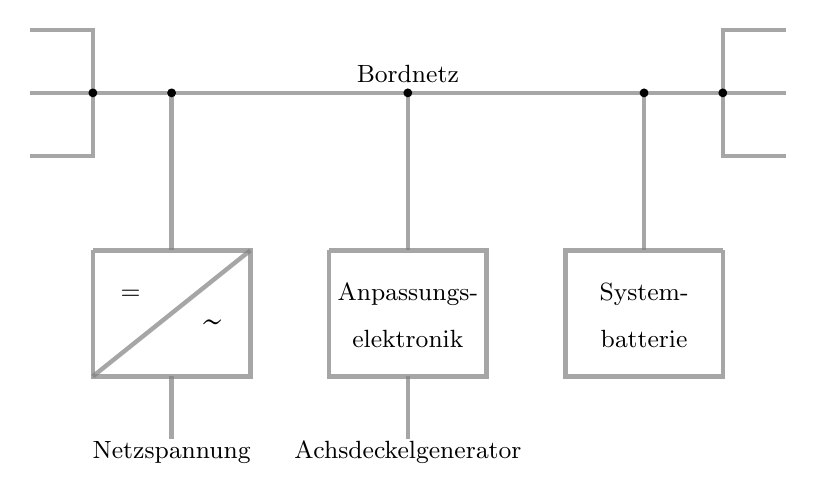
\begin{tikzpicture}[font = \sffamily, scale = 0.8]
\tikzstyle{every node}=[font=\small]
%Bordnetz
\path[wagon] (-6,0) -- (6,0) {};
\node (BN) at (0,0.3) {Bordnetz};
\path[wagon] (-6,1) -- (-5,1) -- (-5,-1) -- (-6,-1){};
\fill(-5,0)circle(2pt);
\path[wagon] (6,1) -- (5,1) -- (5,-1) -- (6,-1){};
\fill(5,0)circle(2pt);

%Netzspannung
\path[wagon] (-3.75,0) -- (-3.75,-2.5) {};
\fill(-3.75,0)circle(2pt);
\path[wagon] (-5,-2.5) -- (-2.5,-2.5) -- (-2.5,-4.5) -- (-5,-4.5) -- (-5,-2.5){};
\path[wagon] (-5,-4.5) -- (-2.5,-2.5) {};
\node (=) at (-4.4, -3.2) {=};
\node (-) at (-3.1, -3.9) {\huge{\textasciitilde}};
\path[wagon] (-3.75,-4.5) -- (-3.75,-5.5) {};
\node (NS) at (-3.75,-5.7) {Netzspannung};

%Achsdeckelgenerator
\path[wagon] (0,0) -- (0,-2.5) {};
\fill(0,0)circle(2pt);
\path[wagon] (-1.25,-2.5) -- (1.25,-2.5) -- (1.25,-4.5) -- (-1.25,-4.5) -- (-1.25,-2.5){};
\node (AE) at (0, -3.2) {Anpassungs-};
\node (AE2) at (0, -3.9) {elektronik};
\path[wagon] (0,-4.5) -- (0,-5.5) {};
\node (NS) at (0,-5.7) {Achsdeckelgenerator};

%Batterie
\path[wagon] (3.75,0) -- (3.75,-2.5) {};
\fill(3.75,0)circle(2pt);
\path[wagon] (5,-2.5) -- (2.5,-2.5) -- (2.5,-4.5) -- (5,-4.5) -- (5,-2.5){};
\node (Bat) at (3.75, -3.2) {System-};
\node (Bat2) at (3.75, -3.9) {batterie};

\end{tikzpicture}